\documentclass[11pt]{article}

\usepackage[margin=0.95in]{geometry}
\usepackage{microtype}
\usepackage{booktabs}
\usepackage{array}
\usepackage{tikz}
\usetikzlibrary{arrows.meta, positioning, fit, calc, backgrounds}
\usepackage{xcolor}
\usepackage{enumitem}
\usepackage[hidelinks]{hyperref}
\usepackage{caption}
\captionsetup{font=small, labelfont=bf}

\definecolor{ink}{HTML}{1D2129}
\definecolor{accent}{HTML}{1A5FB4}
\definecolor{warn}{HTML}{8A4600}
\definecolor{boxfill}{HTML}{E7F0FB}
\definecolor{stofill}{HTML}{FDF3E5}
\definecolor{safefill}{HTML}{E9F5EC}
\definecolor{firewall}{HTML}{B3261E}

\newcommand{\code}[1]{\texttt{#1}}

\title{\vspace{-1.2em}The Skateboard: System Architecture\\
\large Components, Communication, and the Trust Firewall\vspace{-0.4em}}
\author{Companion to \texttt{skateboard.tex}}
\date{July 30, 2026}

\setlength{\parskip}{0.35em}

\begin{document}
\maketitle
\vspace{-1.2em}

\section{What this document decides}

The design note \code{skateboard.tex} says \emph{what} to build. It does not say
\emph{how}. This document makes the concrete choices. It picks the tools. It
draws the parts. It defines how the parts talk to each other. The goal is a
system that runs tonight on one computer, and that grows later to a cluster
without a redesign.

One idea shapes every choice. \textbf{The AI agent is a pure function.} It takes
in source code and a report about what failed. It returns a patch. It has
nothing else. It can reach nothing else. It starts no action on its own.
Everything that builds, runs, measures, or judges the code lives on the far side
of a wall. The wall is enforced by the operating system, not by good manners.
Data crosses the wall. The power to give orders does not.

\section{The components}

The system has six parts. Five are containers. One is a pair of disk volumes.
Table~\ref{tab:components} lists them. Each part has one job. Each part can read
only what it needs. Each part can write only what it owns.

\begin{table}[htbp]
\centering\small
\begin{tabular}{@{}p{0.16\textwidth}p{0.40\textwidth}p{0.18\textwidth}p{0.16\textwidth}@{}}
\toprule
\textbf{Part} & \textbf{Its one job} & \textbf{Networks} & \textbf{Trust} \\
\midrule
\textbf{Orchestrator} & Runs the fixed loop. Decides stage order, retries, and the
strategy ladder. Cleans the failure report. Writes the ledger. It is the only
part that starts anything. & all three & Trusted core \\
\addlinespace
\textbf{Agent\-runner} & Turns one request into one patch, using a chosen model.
Nothing else. & agent, egress & \textbf{Untrusted} \\
\addlinespace
\textbf{Builder} & Compiles the code with fixed flags. Runs it. Proves it ran on
the GPU. Runs the sanitizer. Times it. & build only & Trusted worker \\
\addlinespace
\textbf{Oracle} & Holds the expected answers and the tolerances. Answers one
question: do these numbers match? It runs no code from the agent. & oracle only
& Trusted, sealed \\
\addlinespace
\textbf{Ledger + repo} & An append\-only record and a git repository of every
attempt. Volumes, owned by the orchestrator. & none & Trusted data \\
\addlinespace
\textbf{Model server} \emph{(later)} & Serves local models over a standard API.
& agent only & Untrusted \\
\bottomrule
\end{tabular}
\caption{The six parts. The agent\-runner is the only untrusted part. It shares
no network and no disk with the builder, the oracle, or the ledger.}
\label{tab:components}
\end{table}

\section{How the parts are wired}

Figure~\ref{fig:topology} shows the shape of the system. The orchestrator sits
in the middle. It is the only part on every network. The builder and the oracle
each sit on their own private network. They cannot talk to each other. They can
only answer the orchestrator. The agent\-runner sits above a line we call the
trust firewall. It can reach the internet, so it can call a model. It cannot
reach anything below the line.

\begin{figure}[htbp]
\centering
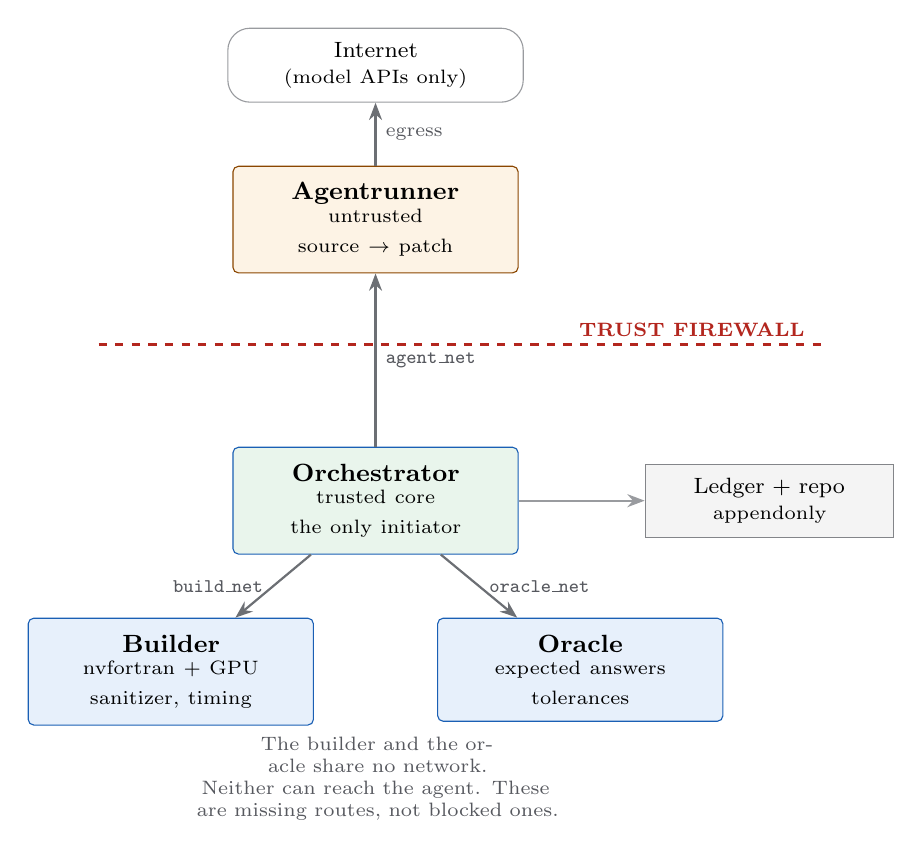
\begin{tikzpicture}[
  node distance=8mm and 12mm,
  box/.style={draw=accent, fill=boxfill, rounded corners=2pt, align=center,
              font=\small, inner sep=6pt, minimum height=11mm, text width=32mm},
  unt/.style={box, draw=warn, fill=stofill},
  safe/.style={box, draw=accent, fill=safefill},
  vol/.style={draw=ink!55, fill=ink!5, align=center, font=\footnotesize,
              inner sep=5pt, text width=28mm, minimum height=9mm},
  cloud/.style={draw=ink!45, fill=white, align=center, font=\footnotesize,
                inner sep=5pt, rounded corners=8pt, text width=34mm},
  arr/.style={-{Stealth[length=2.2mm]}, thick, draw=ink!65},
  lbl/.style={font=\scriptsize, text=ink!75}
]

\node[cloud] (net) {Internet\\ \scriptsize (model APIs only)};
\node[unt, below=of net] (agent) {\textbf{Agent\-runner}\\ \scriptsize untrusted\\ \scriptsize source $\to$ patch};

\node[safe, below=22mm of agent] (orch) {\textbf{Orchestrator}\\ \scriptsize trusted core\\ \scriptsize the only initiator};

\node[vol, right=16mm of orch] (led) {Ledger + repo\\ \scriptsize append\-only};

\node[box, below=of orch, xshift=-26mm] (build) {\textbf{Builder}\\ \scriptsize nvfortran + GPU\\ \scriptsize sanitizer, timing};
\node[box, below=of orch, xshift=26mm] (oracle) {\textbf{Oracle}\\ \scriptsize expected answers\\ \scriptsize tolerances};

% edges
\draw[arr] (agent) -- (net) node[lbl, midway, right] {egress};
\draw[arr] (orch) -- (agent) node[lbl, midway, right] {\code{agent\_net}};
\draw[arr] (orch) -- (build) node[lbl, midway, left] {\code{build\_net}};
\draw[arr] (orch) -- (oracle) node[lbl, midway, right] {\code{oracle\_net}};
\draw[arr, draw=ink!45] (orch) -- (led);

% firewall line
\begin{scope}[on background layer]
  \draw[firewall, dashed, very thick]
    ($(agent.south west)+(-1.7,-0.9)$) -- ($(agent.south east)+(3.9,-0.9)$);
\end{scope}
\node[firewall, font=\scriptsize\bfseries] at ($(agent.south east)+(2.2,-0.72)$)
  {TRUST FIREWALL};

\node[lbl, align=center, text width=52mm] at ($(build.south)!0.5!(oracle.south)+(0,-0.7)$)
  {The builder and the oracle share no network.\\
   Neither can reach the agent. These are missing routes, not blocked ones.};

\end{tikzpicture}
\caption{The topology. The orchestrator is the hub. The agent\-runner is above
the firewall and cannot see the parts below it. The builder and the oracle are
on separate private networks with no route between them.}
\label{fig:topology}
\end{figure}

The wall is real in a plain way. Each network is a separate Docker network. The
Docker daemon writes firewall rules in the Linux kernel for each one. The
agent\-runner has no network card on the builder network or the oracle network.
So it has no address to call. It cannot ask for the held\-out data, because there
is no path to the part that holds it. We do not rely on file permissions. We
rely on the fact that the road does not exist.

A second lock backs up the first. The orchestrator holds a secret token. The
builder and the oracle check that token on every request. Even if a wiring
mistake gave the agent a path, it could not speak the password.

\section{How the parts talk}

Every message is plain HTTP with a JSON body. Arrays of numbers are small here,
so we send them inline. There is no SSH. There is no shared writable disk across
the wall. The orchestrator carries every byte from one part to another, and it
records a hash of each message in the ledger. Table~\ref{tab:edges} lists each
link, who starts it, what it carries, and what it forbids.

\begin{table}[htbp]
\centering\small
\begin{tabular}{@{}p{0.19\textwidth}p{0.37\textwidth}p{0.36\textwidth}@{}}
\toprule
\textbf{Link} & \textbf{What crosses} & \textbf{What is forbidden} \\
\midrule
Orchestrator $\to$ Agent\-runner \code{/v1/attempt} &
Out: the source files, the task, and a clean failure report. In: a unified diff,
notes, and any proposals. &
The agent cannot start a call. It has no second endpoint. The held\-out data is
never named in either direction. A diff that touches a forbidden path is
rejected. \\
\addlinespace
Agent\-runner $\to$ Model &
The prompt, and the model's reply. &
Nothing secret is here to leak. The agent holds only the visible files. \\
\addlinespace
Orchestrator $\to$ Builder \code{/build /run /sanitize /time} &
Out: the patched source, a named flag profile, and input arrays. In: build logs,
output arrays, the count of GPU kernels, and timings. &
The agent cannot pass flags or scripts. The build commands are baked into the
image. The code under test runs with no network. \\
\addlinespace
Orchestrator $\to$ Oracle \code{/compare /policy} &
Out: the output arrays and which dataset. In: pass or fail, and the per\-variable
error for the visible set only. &
There is no write path. Tolerances cannot change over the wire. For the held\-out
set, only pass or fail comes back, never the detailed error. \\
\addlinespace
Orchestrator $\to$ Ledger / repo &
A git branch and one ledger row per attempt, plus saved evidence. &
No other container can see these volumes. \\
\bottomrule
\end{tabular}
\caption{The links between parts. The orchestrator starts every link. The two
links that matter most for safety are the one to the agent and the one to the
oracle. Neither one can carry an order to change how the code is judged.}
\label{tab:edges}
\end{table}

The failure report is the most important message. It is the only way that a
result can shape the next patch. The orchestrator builds this report by hand from
the raw service replies. It never forwards a raw reply. This is where we make
sure the held\-out numbers cannot reach the agent. The rule lives in one small,
trusted place, and a reviewer can read it.

\section{The loop}

Figure~\ref{fig:loop} shows one attempt. The stages run in a fixed order. If a
stage fails, the orchestrator writes a clean report and asks the agent to try
again. There is a hard cap on retries. When the first strategy runs out of tries,
the loop moves to the second strategy. When that runs out, the loop stops and
asks a human. A build that passes is not enough. The code must run on the GPU,
pass the sanitizer, match the expected answers, and then beat the baseline.

\begin{figure}[htbp]
\centering
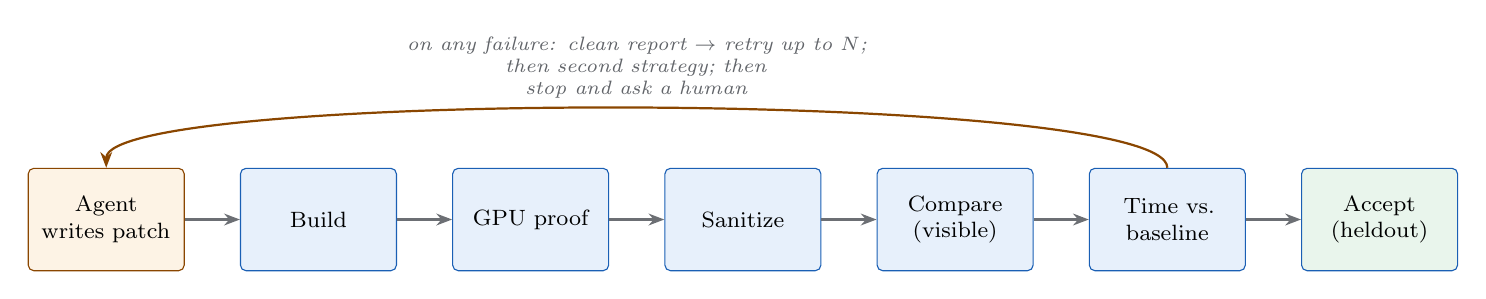
\begin{tikzpicture}[
  node distance=5mm and 7mm,
  st/.style={draw=accent, fill=boxfill, rounded corners=2pt, align=center,
             font=\footnotesize, inner sep=4pt, minimum height=13mm, text width=17mm},
  ag/.style={st, draw=warn, fill=stofill},
  arr/.style={-{Stealth[length=2mm]}, thick, draw=ink!65},
  lbl/.style={font=\scriptsize\itshape, text=ink!70}
]
\node[ag] (agent) {Agent\\ writes patch};
\node[st, right=of agent] (build) {Build};
\node[st, right=of build] (dev) {GPU proof};
\node[st, right=of dev] (san) {Sanitize};
\node[st, right=of san] (cmp) {Compare\\ (visible)};
\node[st, right=of cmp] (time) {Time vs.\\ baseline};
\node[st, right=of time, draw=accent, fill=safefill] (acc) {Accept\\ (held\-out)};

\draw[arr] (agent) -- (build);
\draw[arr] (build) -- (dev);
\draw[arr] (dev) -- (san);
\draw[arr] (san) -- (cmp);
\draw[arr] (cmp) -- (time);
\draw[arr] (time) -- (acc);

\draw[arr, draw=warn]
  ($(time.north)$) .. controls +(0,10mm) and +(0,10mm) .. ($(agent.north)$)
  node[lbl, above, midway, text width=60mm, align=center]
  {on any failure: clean report $\to$ retry up to $N$;\\ then second strategy; then stop and ask a human};
\end{tikzpicture}
\caption{One attempt. The stages run in a fixed order. Passing the build is only
the first step. Only a port that runs on the GPU, is clean, matches the answers,
and beats the baseline reaches the held\-out check.}
\label{fig:loop}
\end{figure}

\section{Why the agent cannot cheat}

The demonstration claims that the agent works under real controls. So we state
plainly why three bad outcomes cannot happen.

\textbf{It cannot edit the tests.} The expected answers and the tolerances live
inside the oracle. The oracle is on a network the agent cannot reach. So ``make
the tests pass'' cannot turn into ``edit the tests.'' The tests are simply out of
reach.

\textbf{It cannot change the build to fake a pass.} The compiler flags, the
build script, and the environment are fixed inside the builder image. The agent's
patch can change only source files. It cannot tell the builder to skip the GPU or
loosen a check.

\textbf{It cannot steal the held\-out data.} The held\-out data sits in one place,
the oracle, on a private network. When the agent's code finally runs, it runs in
the builder with no network at all, so it cannot phone home. The held\-out inputs
reach the code only once, at the final check, after every other gate has passed.
Nothing about the held\-out set, not even its size, ever appears in a message sent
to the agent.

We are honest about the limit. On one computer, these walls stop a
\emph{misbehaving agent}. They are not meant to stop an attacker who breaks the
Linux kernel. That stronger case is the later cluster step, where the oracle
moves to its own machine. The design does not change when we do this. We only
move a box, because every link is already a network call.

\section{Swapping the model}

The system must allow different models. Today it is Claude. Later it may be
Gemini, or a local model like a Qwen coder model. This is easy because the
boundary is the patch, not the model. The agent\-runner exposes one fixed
interface: source in, diff out. Behind that interface sits a small adapter for
each provider.

\begin{itemize}[leftmargin=1.2em, itemsep=0.15em]
  \item The Claude adapter can run a full editing agent inside the container,
  then take the git diff. This keeps Claude's strong multi\-file editing while
  still returning only a patch.
  \item The Gemini adapter and the local\-model adapter both speak a standard
  chat API and are asked to emit a diff.
\end{itemize}

Gemini and local servers both offer an OpenAI\-style endpoint. So one adapter
covers Gemini and every local model. Swapping the model is a change to one config
line. No other part of the system notices. One caution about hardware: a very
large local model does not fit in this GPU's memory, and a resident model would
fight the builder for the GPU during timing. So local models belong on a second
machine, or on the CPU, when we measure speed.

\section{Build our own harness, or use a framework?}

We build our own outer loop. We do not use an agent framework for it. A framework
like LangGraph or AutoGen is built to manage flexible, changing control flow. Our
need is the opposite. We want a fixed order, fixed retries, and a record a
reviewer can replay. That is about three hundred lines of Python, and those lines
\emph{are} the specification. A framework would also sit on the trust boundary,
and any clever feature it adds, like a tool loop the model did not expect, is a
hole in the wall. We keep the trusted core small, plain, and fully ours.

We still use provider libraries, but only inside the adapters, where they are a
private detail. The one exception worth naming is that the Claude adapter may use
Claude's own agent tools inside its container. That is safe, because the
container is already untrusted and already walled off.

\section{The GPU container}

The builder is a long\-running service. It is not a container we reach into with
a shell. This matters for safety. Reaching in with a shell would force the
orchestrator to hold the Docker control socket, and that socket is as powerful as
root on the whole machine. A service avoids that. It also fixes the exact set of
commands that can ever run on the GPU, in one file, which is what we want.

The builder image is the NVIDIA HPC SDK image from NVIDIA's registry. It ships
the \code{nvfortran} compiler, the \code{compute\-sanitizer}, and the
\code{nsys} profiler together. So the build gate, the GPU proof, the sanitizer
gate, and the timing all live in one container with one pinned version. That
pinned version is a single line in the compose file, which is also how we make
the whole system easy to rebuild elsewhere.

\section{Requirements}

The architecture must meet these requirements.

\begin{itemize}[leftmargin=1.2em, itemsep=0.15em]
  \item \textbf{Portable.} \code{git clone} and \code{docker compose up} bring
  the whole system up on any Linux host with an NVIDIA GPU and the container
  toolkit. Every tool version is pinned as an image tag.
  \item \textbf{Isolated.} The agent shares no network and no disk with the
  builder, the oracle, or the ledger. The rule is enforced by the kernel. No
  container holds the Docker socket. The held\-out data lives in one place.
  \item \textbf{Least message.} No message sent to the agent can name or carry
  the held\-out data. This is enforced by the shape of the API, not by policy
  alone.
  \item \textbf{Deterministic loop.} The same inputs give the same stage order
  and the same record. The only random part is the model's patch. So we
  \emph{measure} repeatability by rerunning from a clean checkout three times,
  rather than claim it.
  \item \textbf{Auditable.} The ledger is append\-only. Every message across the
  wall is hashed into it. Every claim in the final report traces to a saved
  artifact.
  \item \textbf{Honest speed.} A timing run needs the GPU to itself, a
  full\-size input, and repeated runs reported as a spread.
  \item \textbf{Swappable model.} The model is chosen by config, with no change
  to any other part.
  \item \textbf{Grows without a redesign.} Moving the oracle or the builder to
  another machine changes a URL, not a contract.
\end{itemize}

\section{Tonight, and later}

\textbf{Tonight.} The full shape above is also the smallest honest version,
because the walls are the whole point. What makes it fit in one evening is that
each service is thin. The builder wraps a handful of commands. The oracle is a
short piece of numpy behind three endpoints. The agent\-runner wraps one model
call. The orchestrator is the loop. Tonight we run one model, Claude. We use a
token for auth and skip TLS, because the networks are private. We send arrays as
inline JSON. We gate on the memory and race checks, and we log the third check.

\textbf{One host step is needed first.} The machine does not yet have the NVIDIA
container toolkit, so a container cannot see the GPU. A short install with
\code{sudo}, plus \code{nvidia\-ctk runtime configure} and a Docker restart,
fixes this. Everything else is already present. The large compiler image is the
slow download, so we start it first.

\textbf{Later.} Each of these drops in without a redesign: the Gemini and local
adapters and a local model server; an outbound proxy that limits where the agent
can connect; the ledger as its own service; TLS and per\-service tokens; tighter
container limits; and finally the cluster split, where the oracle moves to its
own machine. That last step is a URL change, and that is the payoff for refusing
SSH and shared disks now.

The one sentence to remember is this. Last night's boundary was a file
permission. This design's boundaries are roads that do not exist and messages
that cannot say the forbidden thing. Both hold when we move from one laptop to a
cluster, because neither depends on the machine.

\end{document}
